\subsection{Shell - a console de comandos}
O Mongo Shell, também conhecida como Console de Comandos, utiliza uma interatividade entre comandos JavaScript e o MongoDB. Aqui é possível realizar operações administrativas como consultas ou manutenções de dados.

Mostrar as bases de dados existentes: \\
\codigo{> show dbs}

Criar (ou mudar) a base de dados para a atual: \\
\codigo{> use nome\_base}

Mostrar as coleções existentes na base de dados atual: \\
\codigo{> show collections}

* \textbf{db} deixar como está pois é uma variável interna que aponta para a base de dados atual e \textbf{col} deve ser modificada para o nome da coleção nas ações abaixo.

Inserir (ou alterar caso o objeto tenha sido chamado anteriormente) um documento em uma coleção (se a coleção não existe será criada) na base de dados corrente: \\
\codigo{> db.col.save(\{"campo1":"valor1", ..., "campoN":"valorN"\})} 

Listar os documentos de uma coleção existente na base de dados atual: \\
\codigo{> db.col.find()}

Listar um documento específico de uma coleção existente na base de dados atual: \\
\codigo{> db.col.find(\{"campo":"valor"\})}

Adicionar uma nova coluna: \\
\codigo{> db.col.update(\{\}, \{"\$set":\{"campo":"valor"\}\}, \{upsert:false, multi:false\})}

Eliminar documento(s) de uma coleção existente na base de dados atual: \\
\codigo{> db.col.remove(\{campo:valor\})}

Apagar uma coleção existente na base de dados atual: \\
\codigo{> db.col.drop()}

Apagar a base de dados atual: \\
\codigo{> db.dropDatabase()}

Se percebemos bem a única diferença do MongoDB para bancos relacionais é entendermos como é o relacionamento entre os objetos:
\begin{figure}[H]
	\centering
	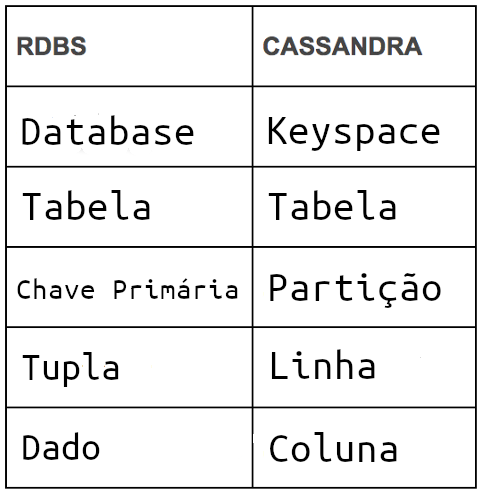
\includegraphics[width=0.5\textwidth]{imagens/comparativo.png}
	\caption{Comparativo entre os objetos do MongoDB e SQL}
\end{figure}

Para conhecer mais comandos do Shell, podemos acessar o seguinte endereço: \url{https://docs.mongodb.org/manual/mongo/}.